%duvida 1: qual melhor pessoa para usar em frazes
%   nessa etapa precisamos (ingles)
%   nessa etapa é preciso
%   nessa etapa precisei
%   nessa etapa foi necessário       usar essa

%Conjunto de equações, recomendação do emílio
%\begin{align}
%    A \in Z^{2} \\
%    mix(A, B, c) &= (1-c) * A + c*B \\
%    mix(A, B, c) &= (1-c) * A + c*B \\
%\end{align}

\chapter{Implementação}

%Essa seção não é muito relevante para o resultado final, não sei se escrevo ela
\section{Configuração do Ambiente}

%Mover para fundamentação teórica
\subsection{Usando os Buffers do OpenGL e GLSL}

\subsubsection{Descrição dos vértices}
Um vértice $v$ é um conjunto de informações relacionadas a alguma unidade, %DEBUG: trocar o termo unidade
a informação necessária para este projeto é posição no espaço, então cada vértice
vai possuir uma posição notada por $v.pos$, e $v.pos$ é composto por 
$\{x, y, z\} \in \mathbb{Q}^3$. Um segundo dado será usado, a cor, vai ser uma 
informação auxiliar, usada para melhor vizialização dos resultados, 
representada por $\{r, g, b \in \mathbb{Q}:0 \leq r, g, b \leq 1\}$ onde cada um desses
vai referir a proporção de vermelho, verde e azul respectivamente.

\subsubsection{Implementação do sistema de Navegação}

\section{\textit{Terrain chunk}}
Representando um fragmento do terreno, o objeto \textit{Terrain chunk} é responsavel
por gerar uma malha para o terreno com $k^2$ vértices, o construtor pode receber 
a seguinte tupla para inicialização: 
$terrainChunk(seed, \Delta{v}, k, x_{s}, z_{s}, b, l)$
%referenciar as fatias do fernando
\begin{itemize}
    \item $seed \in \mathbb{N}$ representa a semente para começar o motor de números
    pseudo-aleatórios;
    \item $\Delta{v} \in \mathbb{Q}:0 < \Delta{v} < l/2$ é a distância entre vértices adjeacentes na
    projeção do plano $X \times Z$;
    \item $k \in \mathbb{N}>4$ é a quantidade de vértices em cada coluna ou 
    linha, a malha tem $k^2$ vértices;
    \item $x_{s} \in \mathbb{Q}:$ é o valor inicial no eixo $X$;
    \item $z_{s} \in \mathbb{Q}:$ é o valor inicial no eixo $Z$;
    \item $b \in \mathbb{N}>4:$ a área da região de cada bioma vai ser $b^2$;
    \item $l \in \mathbb{N}:1 < l < b/2$ distância para fronteira entre biomas ser interpolada.
\end{itemize}


Em cada execução da iplementação os valores que podem mudar de uma chunk para 
outra são apenas $x_{s}$ e $z_{s}$. Uma maneira de conseguir gerar terreno sobre demanda
é usando a localização da camera $(x_{c}, y_{c}, z_{c})$, quando ela se
aproxima de alguma borda da chunk atual
uma \textit{thread} é acionada pedidndo para calcular uma nova chunk, com os parâmetros
$x_{s} = x_{c}/\Delta{v} - k/2$ e $z_{s} = z_{c}/\Delta{v} - k/2$, assim que ela
estiver calculada a mesma começa a ser renderizada, substituindo a chunk anterior.
Antes de renderizar alguma chunk é necessário fazer uma translação com o vetor direção 
$(x_{s} * \Delta{v}, 0.0, z_{s} * \Delta{v})$, já que internamente cada chunk vai 
da posição $(0, 0)$ até $(\Delta{v}*(k-1), \Delta{v}*(k-1))$, mas representando a área 
no mundo $(x_{s}, z_{s})$ até $(x_{s} + \Delta{v}*(k-1), z_{s} + \Delta{v}*(k-1))$

\section{Criando Malha de Triângulos}
A maneira que um jogo renderiza seu terreno no final das contas é sobre uma
malha, uma malha é um conjunto de vértices que podem representar fragmentos
de uma superfície do terreno.

Para representar um segmento de plano precisamos de pelo menos $3$ vértices, 
já que com dois podemos apenas representar segmentos de retas. Um plano precisar
ter um mesmo vetor normal para todo o plano.

A malha segue pelo plano $X \times Z$, e cada vértice do plano vai ter uma altura
$y$ definida mais tarde por ruído. Se quisermos que o conjunto de pontos pertença
ao memos segmento de plano precisamos que os quatro pontos respeitem a mesma
equação do plano.%colocar referêrencia da malha de triângulos

Se usarmos como plano $4$ pontos em $\mathbb{Q}^3$
\begin{equation}\label{comp_sign_inter_sem_peso_aux}
    P = \{p_{0}(0, y_{0}, 0), p_{1}(0, y_{1}, 1), p_{2}(1, y_{2}, 0), p_{3}(1, y_{3}, 1)\}
\end{equation}
Para montar a equação do plano temos $\{y_{0}, y_{1}, y_{2}\}$ como valores livres e $y_{3}$
vai depender dos valores de $\{p_{0}, p_{1}, p_{2}\}, x_{3} e z_{3}$

%Aqui vai o cálculo da equação do plano ou do vetor normal para mostrar o que
%acabei de afirmar acima
%Calculando o vetor normal associado ao plano formado por $\{v0, v1, v2\}$
%$v0v1 = (0, y1-y0, 1)$
%$v0v2 = (1, y2-y0, 0)$

mas não é isso o objetivo, já que o ruído pode retornar valores para $y_{3}$
que não respeitem a equação do plano queremos que todos os pontos tenha valores de $y$
livres, portanto, será uma malha de triângulos. Então pro conjunto de vértices
acima temos dois triângulos associados:
$T_{1} = \{p_{0}, p_{1}, p_{2}\}, T_{2} = \{p_{3}, p_{1}, p_{2}\}$, que podem ser
vizualizados na figura \ref{fig:t1t2}. 
Desta maneira temos todos os pontos com $y$ livre.

\begin{figure}[H]
    \centering
    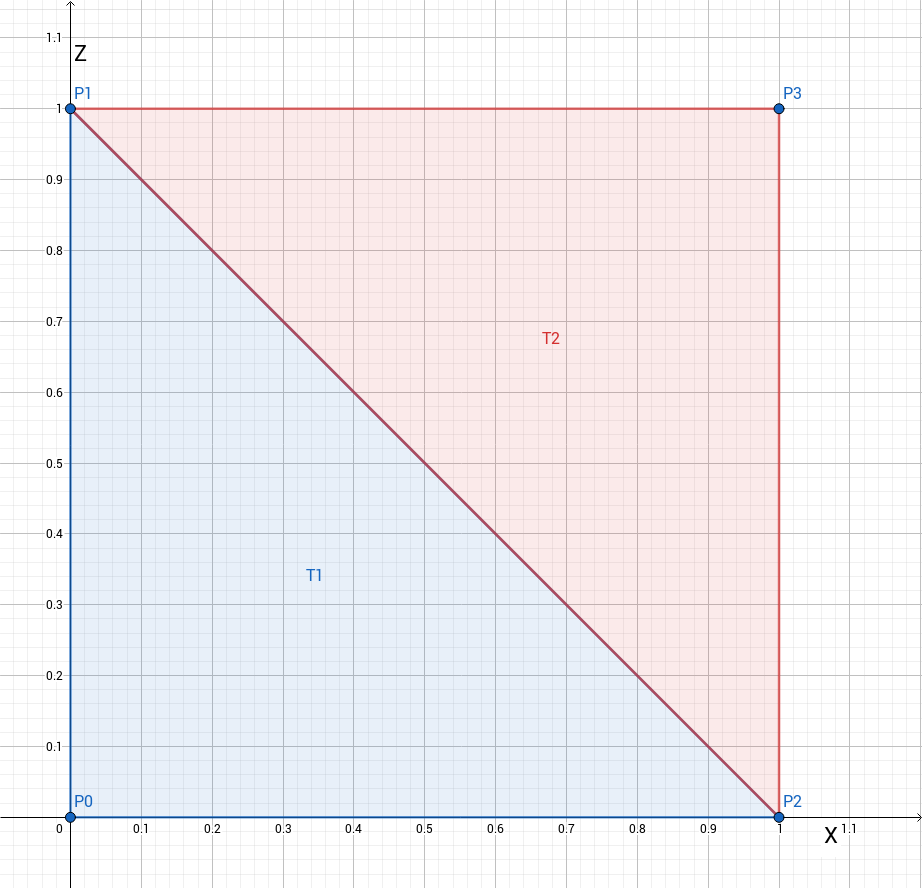
\includegraphics[width=0.5\textwidth]{figuras/t1t2.png}
    \caption{$T_{1}$ e $T_{2}$ projetados em $X \times Z$}
    \label{fig:t1t2}
\end{figure}


Então para montar um grid renderizavel usamos o algoritmo \ref{alg:genVectors}
$V$ é a estrutura que armazena os vértices, de $v_{0}$ até $v_{k^2-1}$ 
$E$ é a estrutura que armazena os índices, já que o \textit{OpenGL} precisa
saber a ordem de desenhar cada triângulo e quais vértices fazem parte dele, 
cada elemento de $e_{i} \in \mathbb{N}$ e a estrutura vai de $e_{0}$ até $e_{(k-1)^2 * 6 - 1}$.

A função \textit{$hEvaluation(x, z)$}, será comentada mais adiante, ela retorna uma estrutura
com a altura e cor para algum ponto $(x, z)$.
 
\begin{algorithm}[H]\label{alg:genVectors}
    $|V| = k^2$\;
    \For{$i=0$ \KwTo $k-1$}{
        \For{$j=0$ \KwTo $k-1$}{
            $v_{i*k + j}.pos = (\Delta_{v} * i, hEvaluation(x_{s} + i, z_{s} + j).h, \Delta{v} * j)$\;
            $v_{i*k + j}.cor = hEvaluation(x_{s} + i, z_{s} + j).c$
        }
    }
    $|E| = (k-1)^2*6$\;
    \For{$i=0$ \KwTo $k-2$}{
        \For{$j=0$ \KwTo $k-2$}{
            //posições em $V$ do primeio triângulo\;
            $e_{(i*(k-1)+j)*6} = (i*k +j)$\;
            $e_{(i*(k-1)+j)*6+1} = (i*k +j+1)$\;
            $e_{(i*(k-1)+j)*6+2} = ((i+1)*k +j)$\;
            //posições em $V$ do segundo triângulo\;
            $e_{(i*(k-1)+j)*6+3} = ((i+1)*k +j+1)$\;
            $e_{(i*(k-1)+j)*6+4} = (i*k +j+1)$\;
            $e_{(i*(k-1)+j)*6+5} = ((i+1)*k +j)$\;
        }
    }
    \caption{Construção da coleção de vértices e índices.}
\end{algorithm}

Considerando que \textit{$hEvaluation(x, z)$} retorne sempre a cor branca
e a altura $0.0$, por hora os parâmetros $seed, b, l$ não terão influência, os mesmos 
só serão usados na função \textit{$hEvaluation$}, e fixando os parêmtros: $x_{s}, z_{s} = 0$, 
podemos analisar a influencia de $k$ e $\Delta_{v}$ nas figuras \ref{fig:parametrosGrid}

\begin{figure}[H]
     \centering
     \subfloat[][$k = 4, \Delta_{v} = 0.5$]{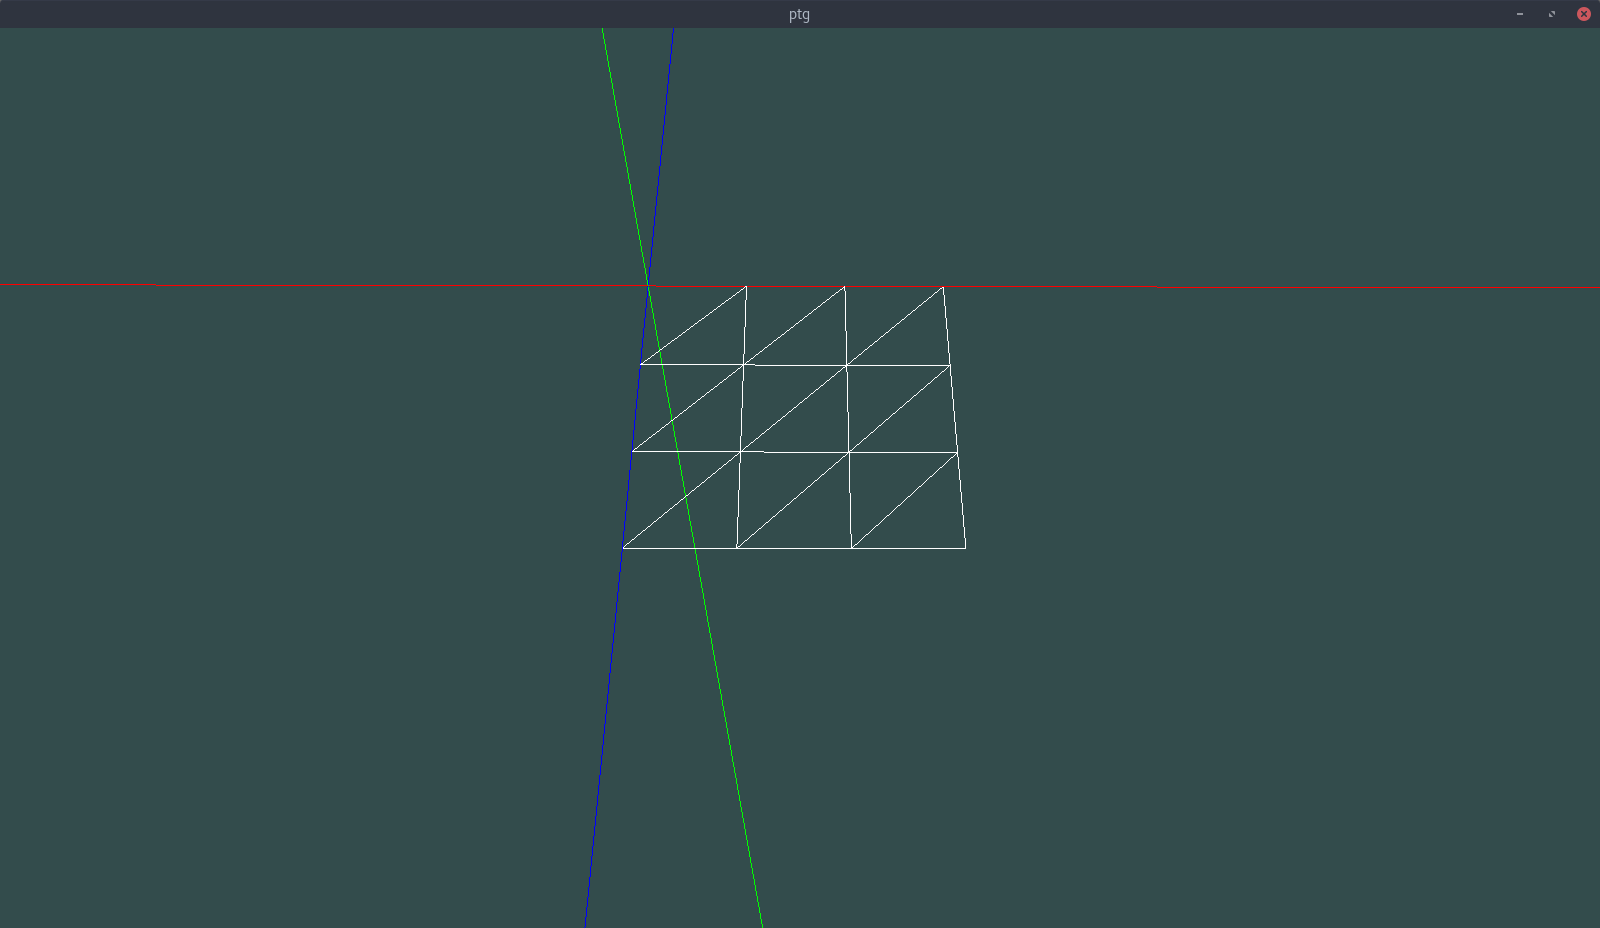
\includegraphics[width=0.3\textwidth]{figuras/k4d5.png}\label{fig:k4d5}}\hspace{0.1cm}
     \subfloat[][$k = 8, \Delta_{v} = 0.5$]{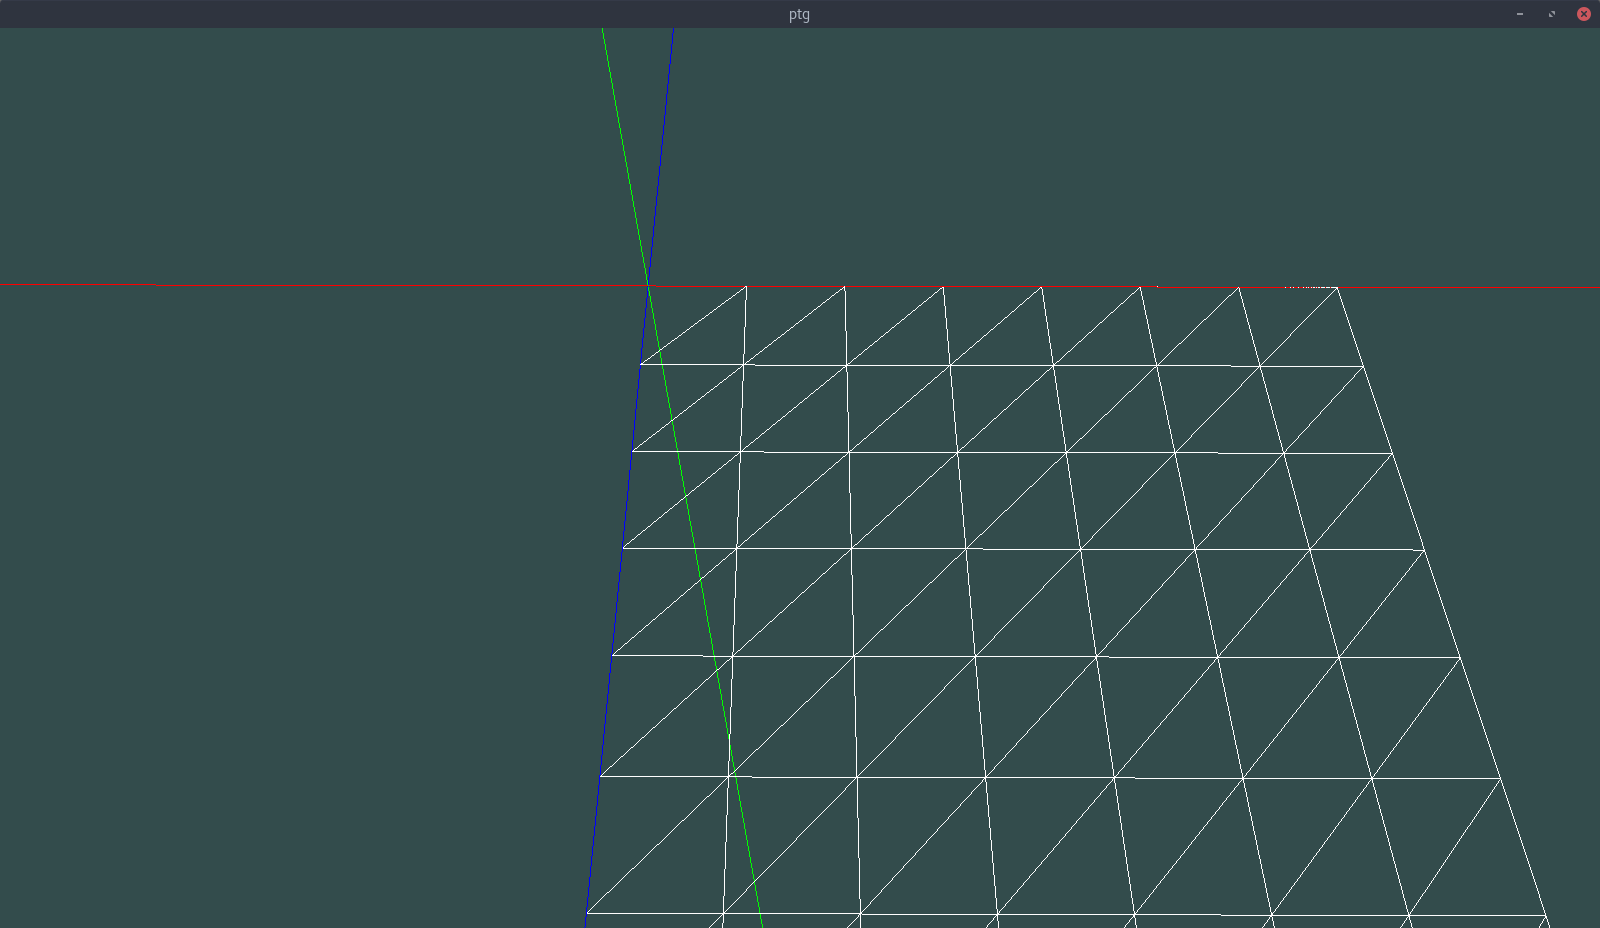
\includegraphics[width=0.3\textwidth]{figuras/k8d5.png}\label{fig:k8d5}}\hspace{0.1cm}
     \subfloat[][$k = 8, \Delta_{v} = 0.25$]{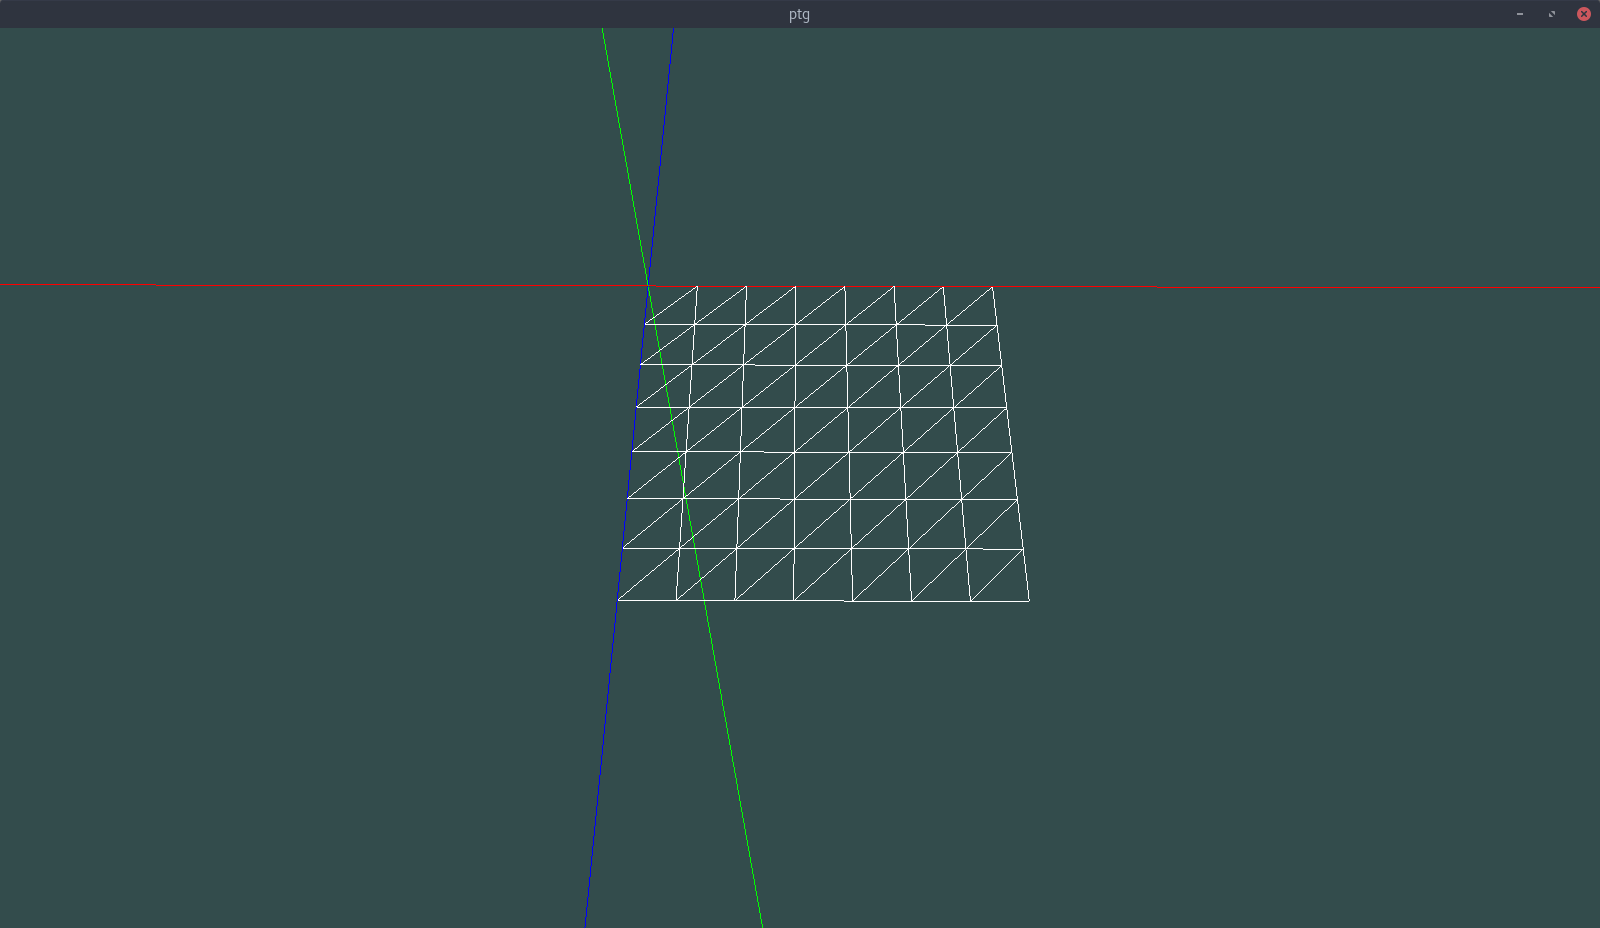
\includegraphics[width=0.3\textwidth]{figuras/k8d25.png}\label{fig:k8d25}}
     \caption{Comparando os parâmetros $k$ e $\Delta_{v}$}
     \label{fig:parametrosGrid}
     % usar \hspace{0.1cm}, é gambiarra mas funciona
\end{figure}


\section{Aplicando Ruído de Perlin nos Vértices}


\begin{figure}[H]
    \centering
    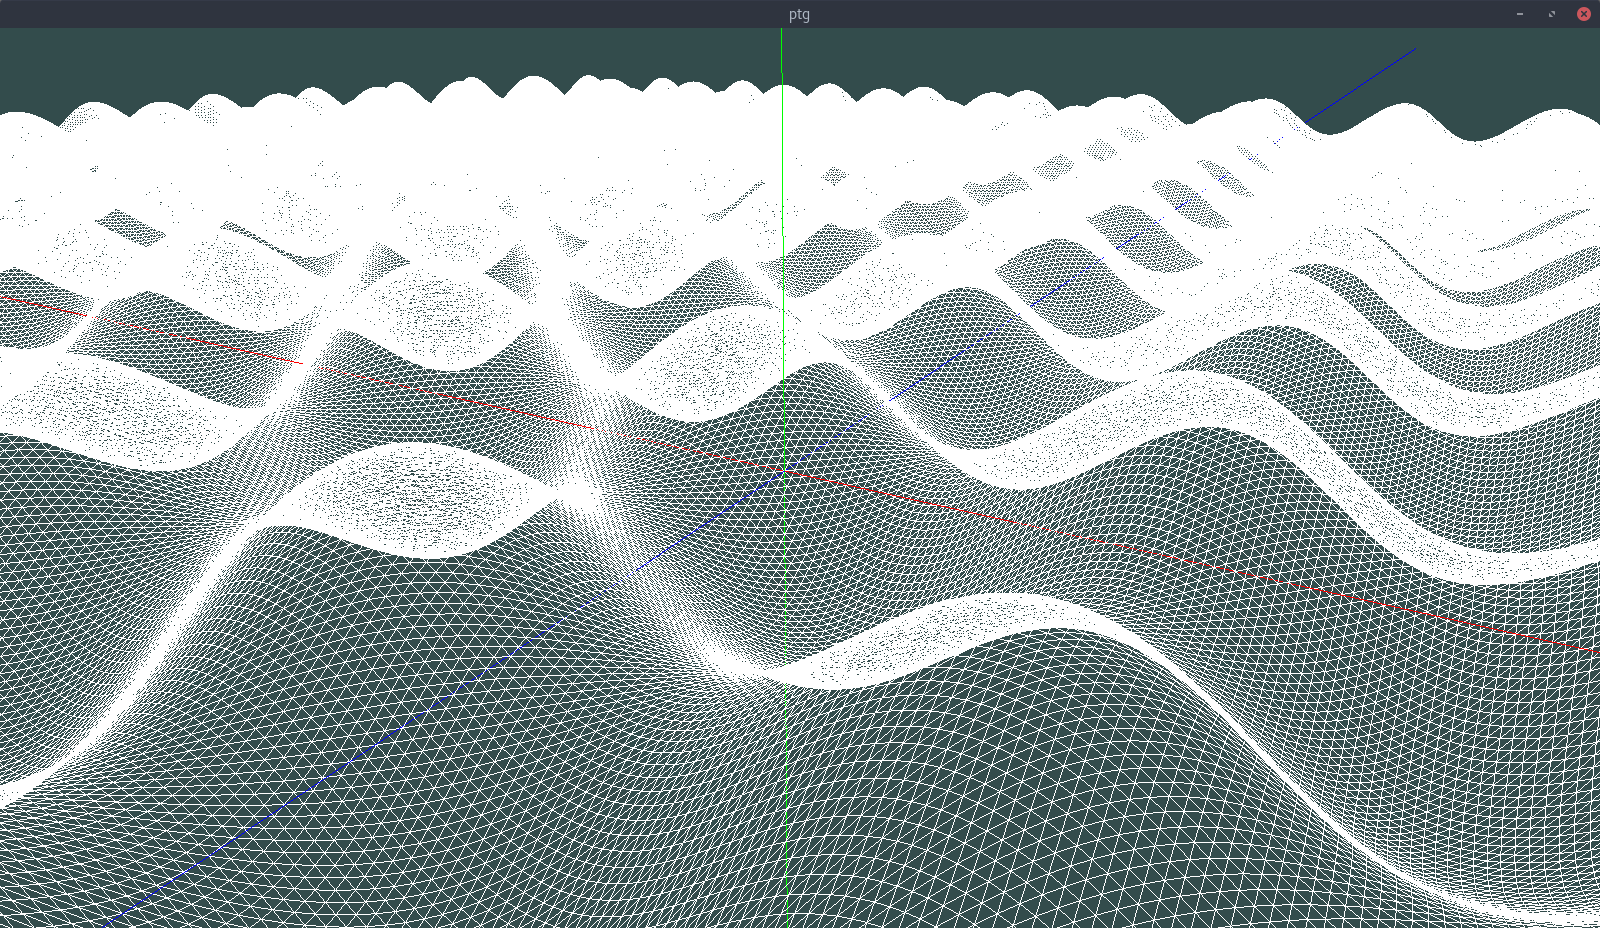
\includegraphics[width=0.75\textwidth]{figuras/sssins.png}
    \caption{Se a altura for $(sin(x/10) + sin(z/10)) * 4$}
    \label{fig:sssins}
\end{figure}

Usando ruído de Perlin...

$amp$ é a amplitude escalar do terreno.\\
$f$ é a frequência;\\
$fxz$ é a frequência relativa a malha;\\
$fxz = k/f$\\
$Altura = PerlinNoise(x/fxz, z/fxz, Octaves) * amp$\\

Usando $f = 8$, $amp = 30, seed = 15$ e variando o número de oitavas.

\begin{figure}[H]
     \centering
     \subfloat[][$Octaves = 1$]{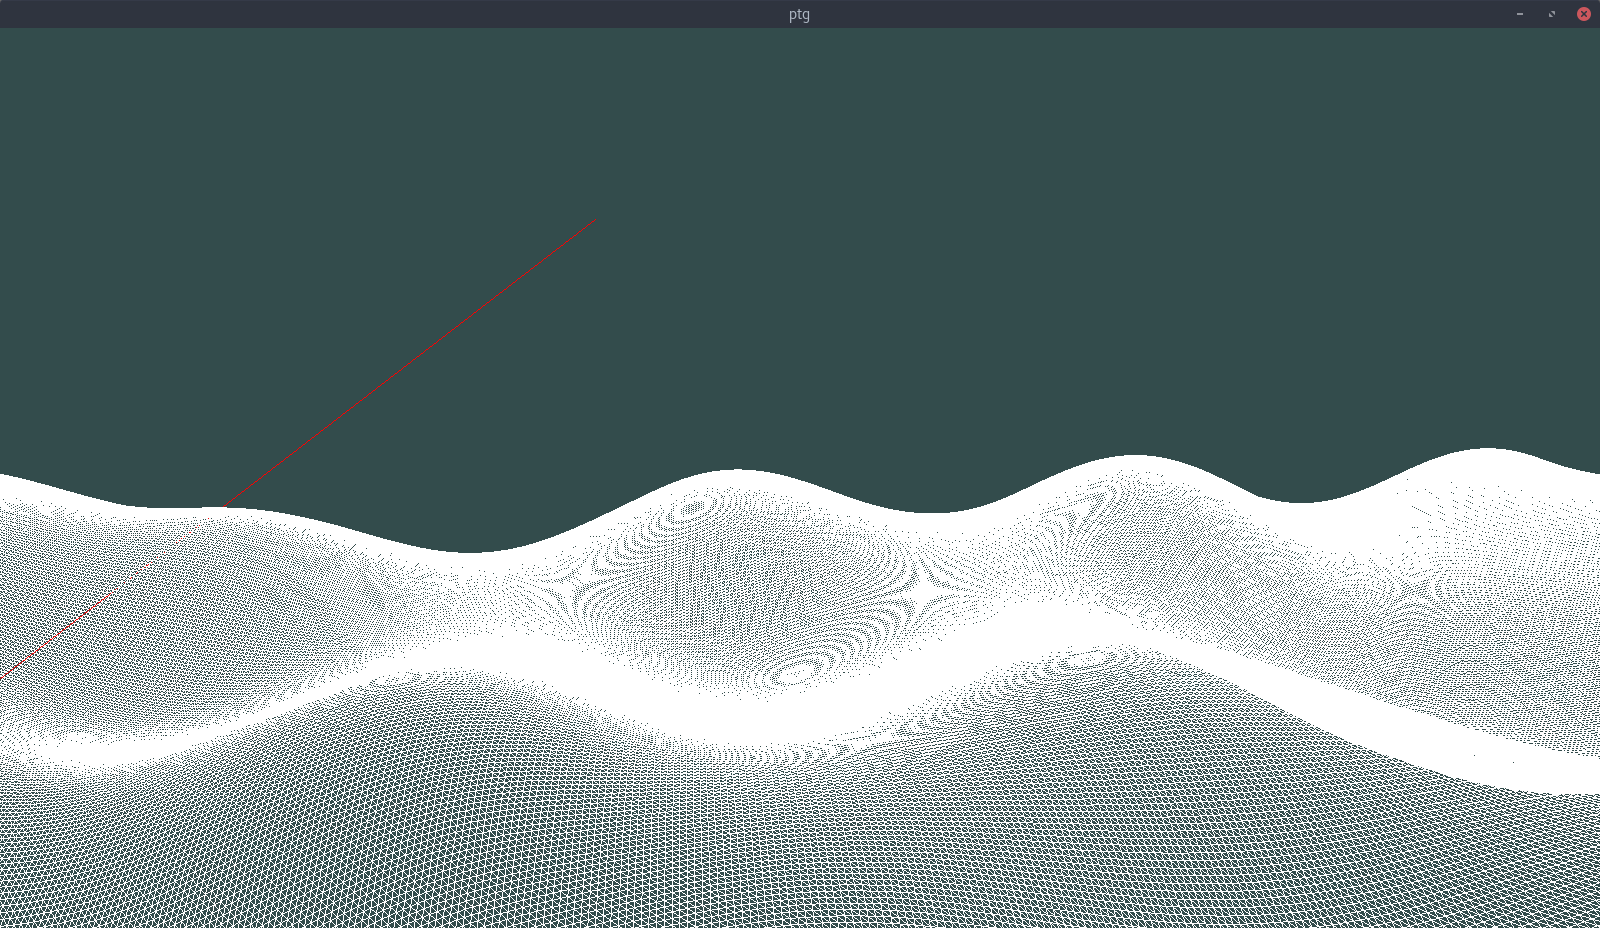
\includegraphics[width=0.3\textwidth]{figuras/octaves1.png}\label{fig:octaves1}}\hspace{0.1cm}
     \subfloat[][$Octaves = 4$]{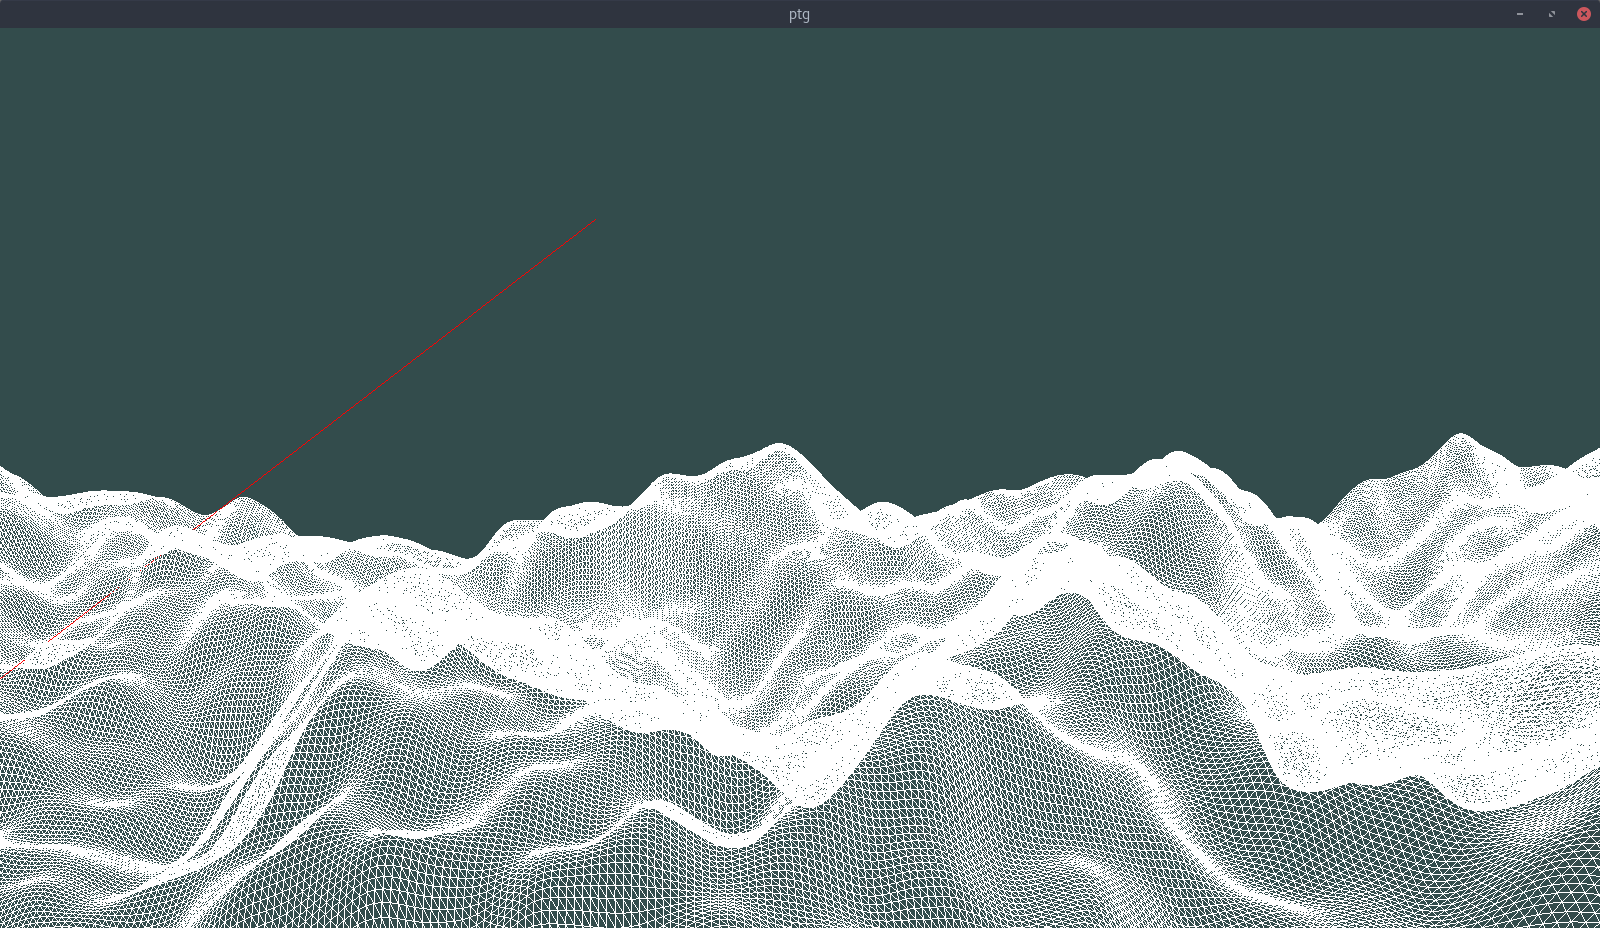
\includegraphics[width=0.3\textwidth]{figuras/octaves4.png}\label{fig:octaves4}}\hspace{0.1cm}
     \subfloat[][$Octaves = 16$]{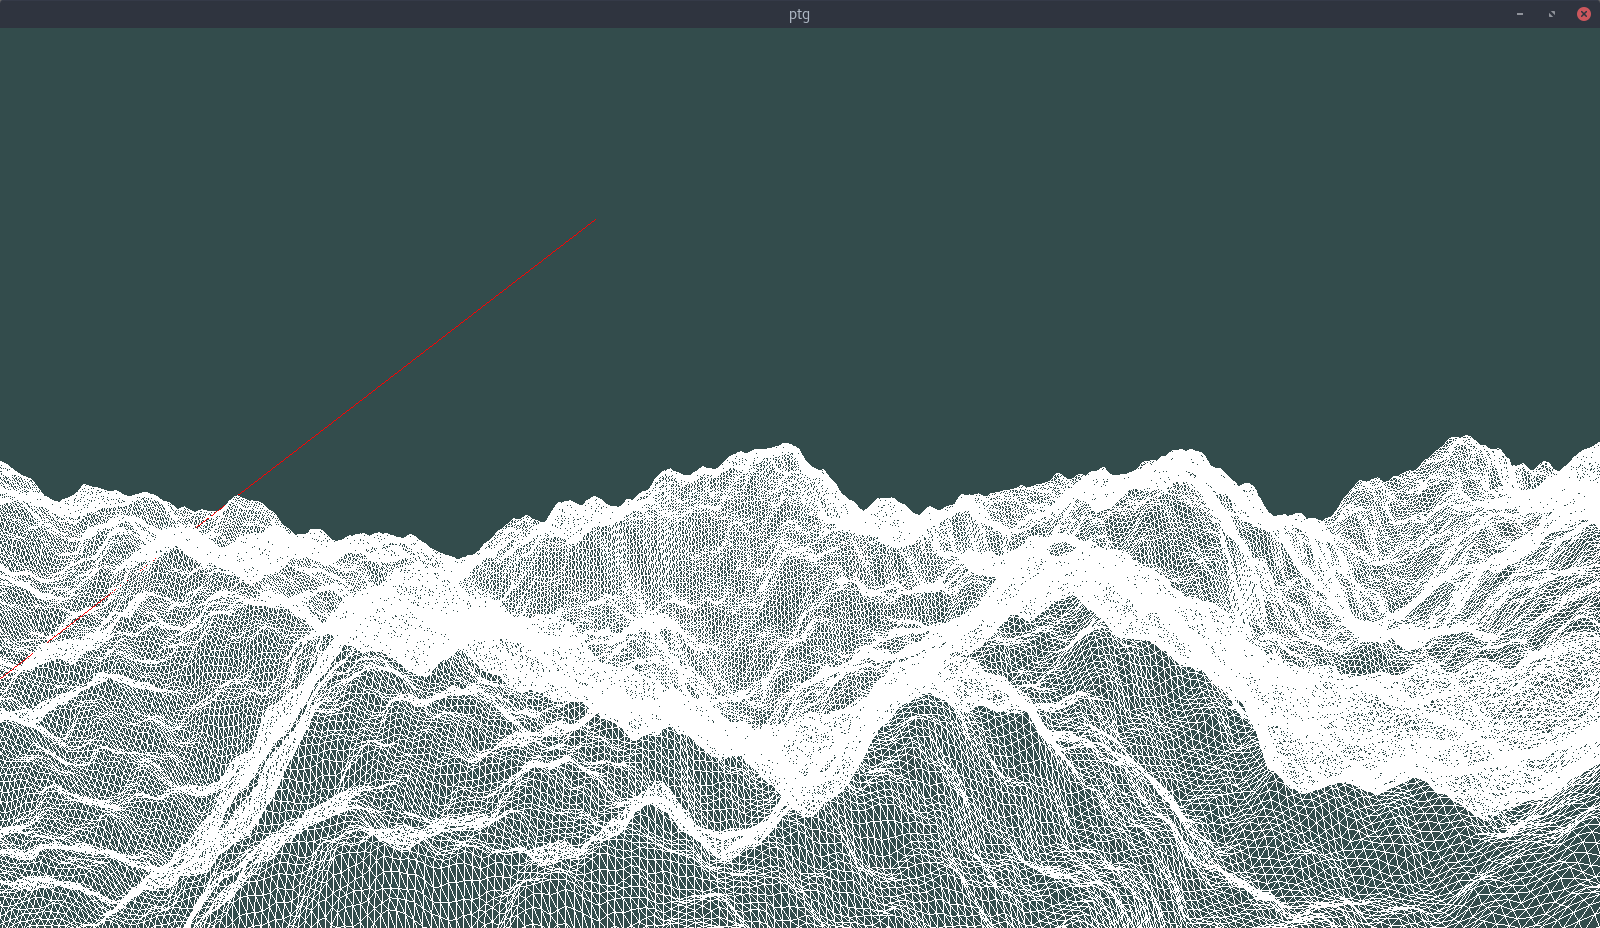
\includegraphics[width=0.3\textwidth]{figuras/octaves16.png}\label{fig:octaves16}}
     \caption{Comparando influência das oitavas.}
     \label{fig:parametrosOctaves}
     % usar \hspace{0.1cm}, é gambiarra mas funciona
\end{figure}

Usando $amp = 30$ e $Octaves = 8, seed = 15$ e variando a frequência.

\begin{figure}[H]
     \centering
     \subfloat[][$f = 1$]{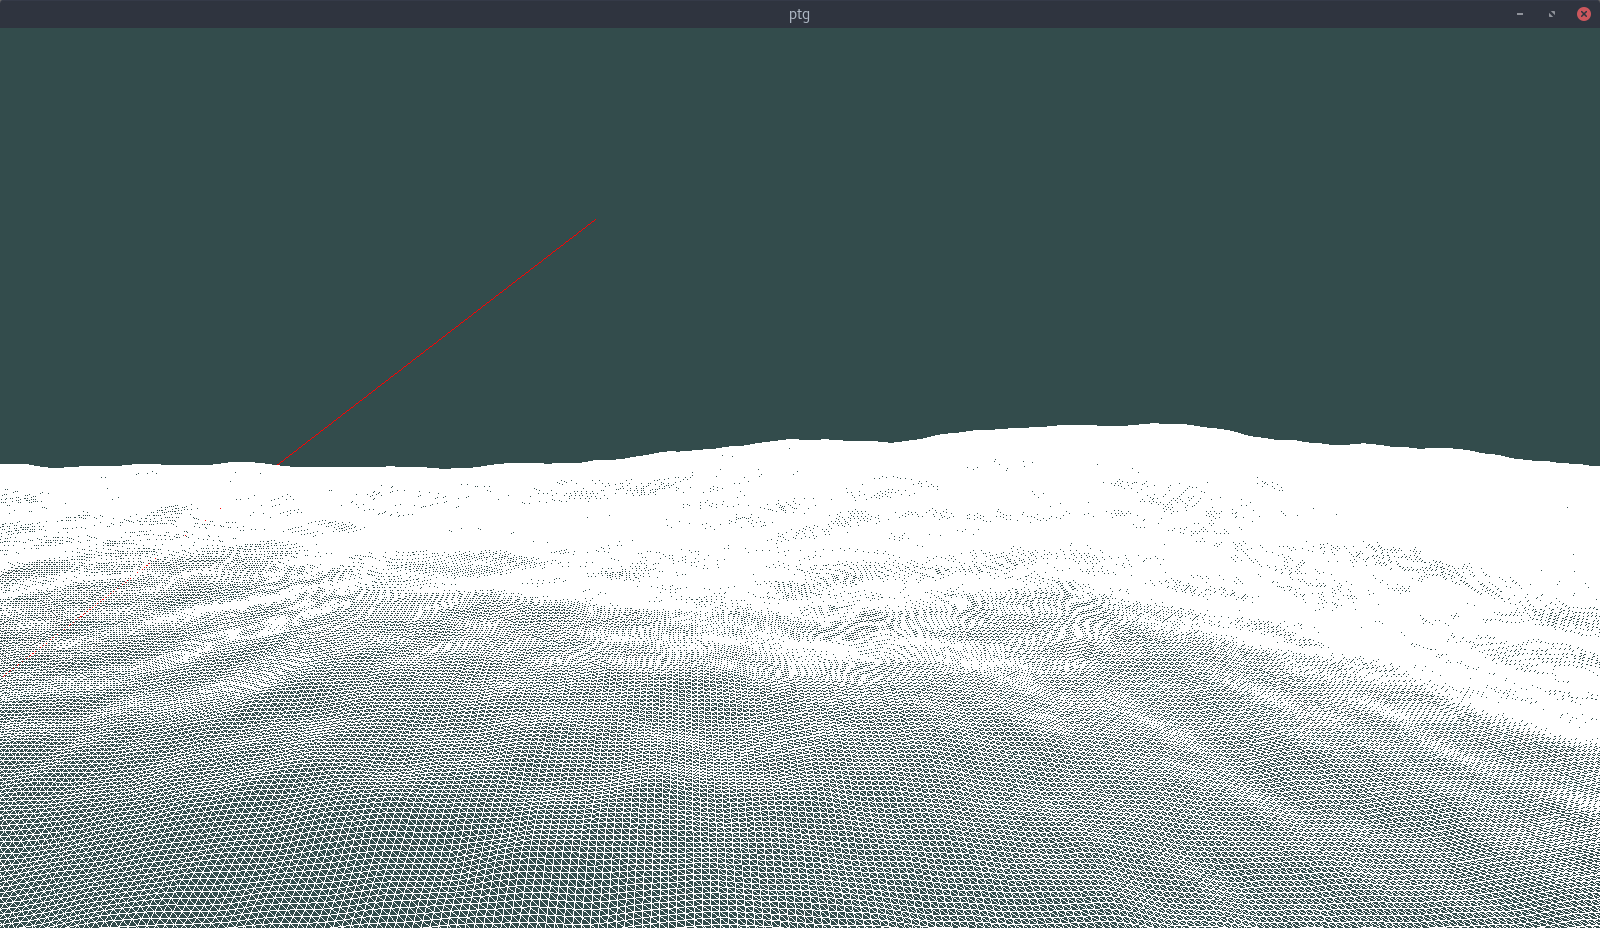
\includegraphics[width=0.3\textwidth]{figuras/freq1.png}\label{fig:freq1}}\hspace{0.1cm}
     \subfloat[][$f = 4$]{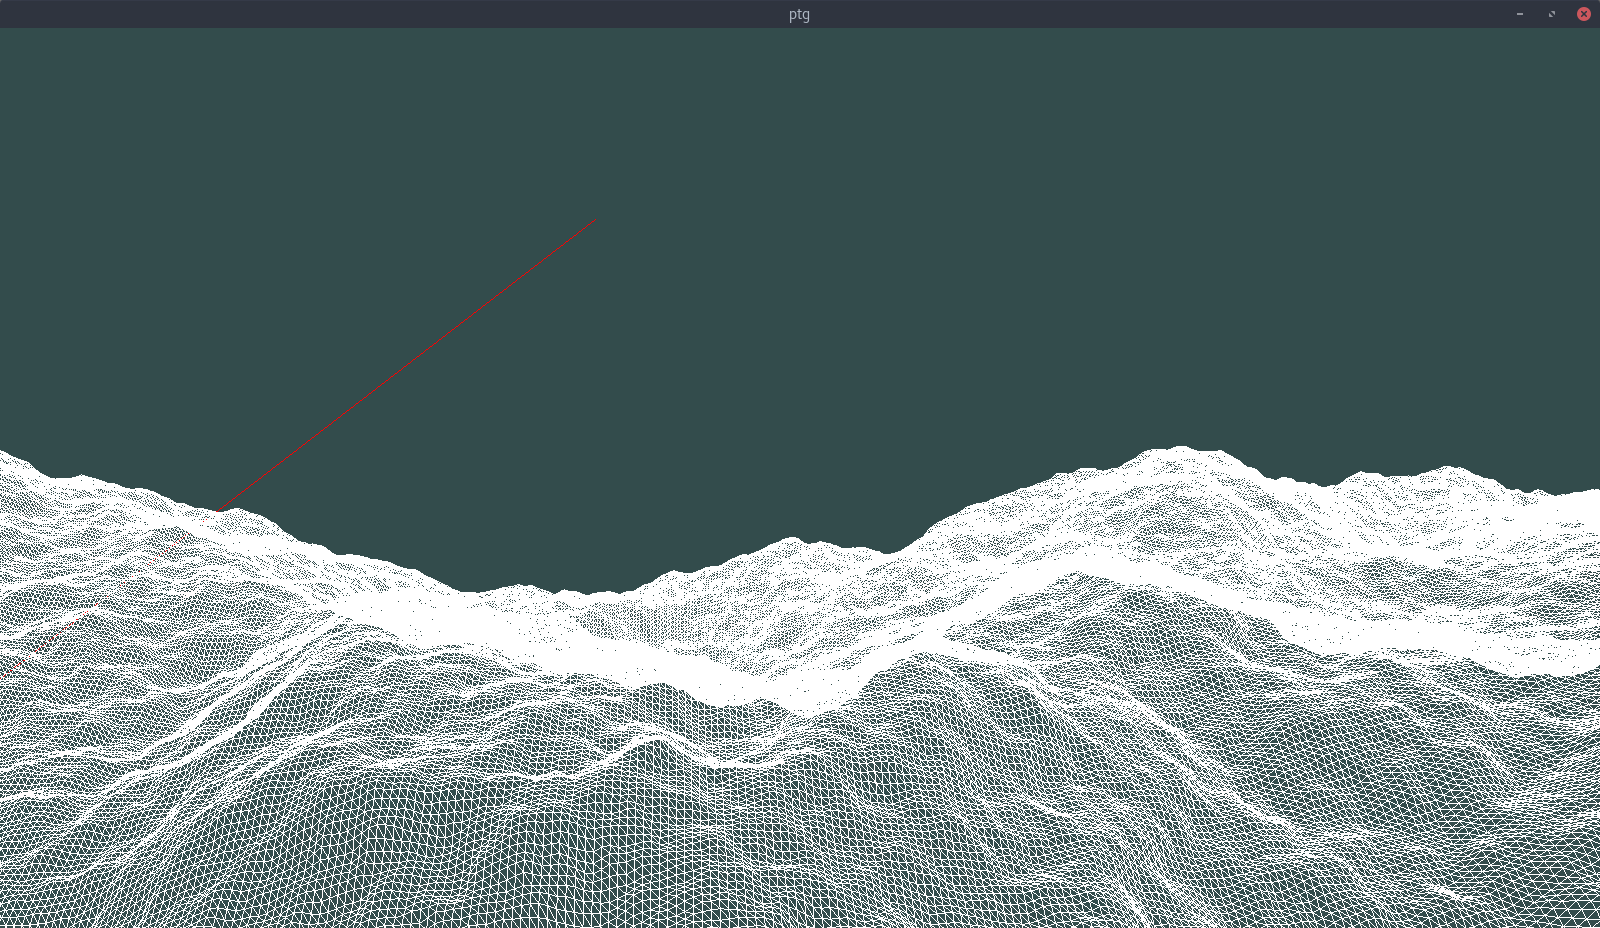
\includegraphics[width=0.3\textwidth]{figuras/freq4.png}\label{fig:freq4}}\hspace{0.1cm}
     \subfloat[][$f = 16$]{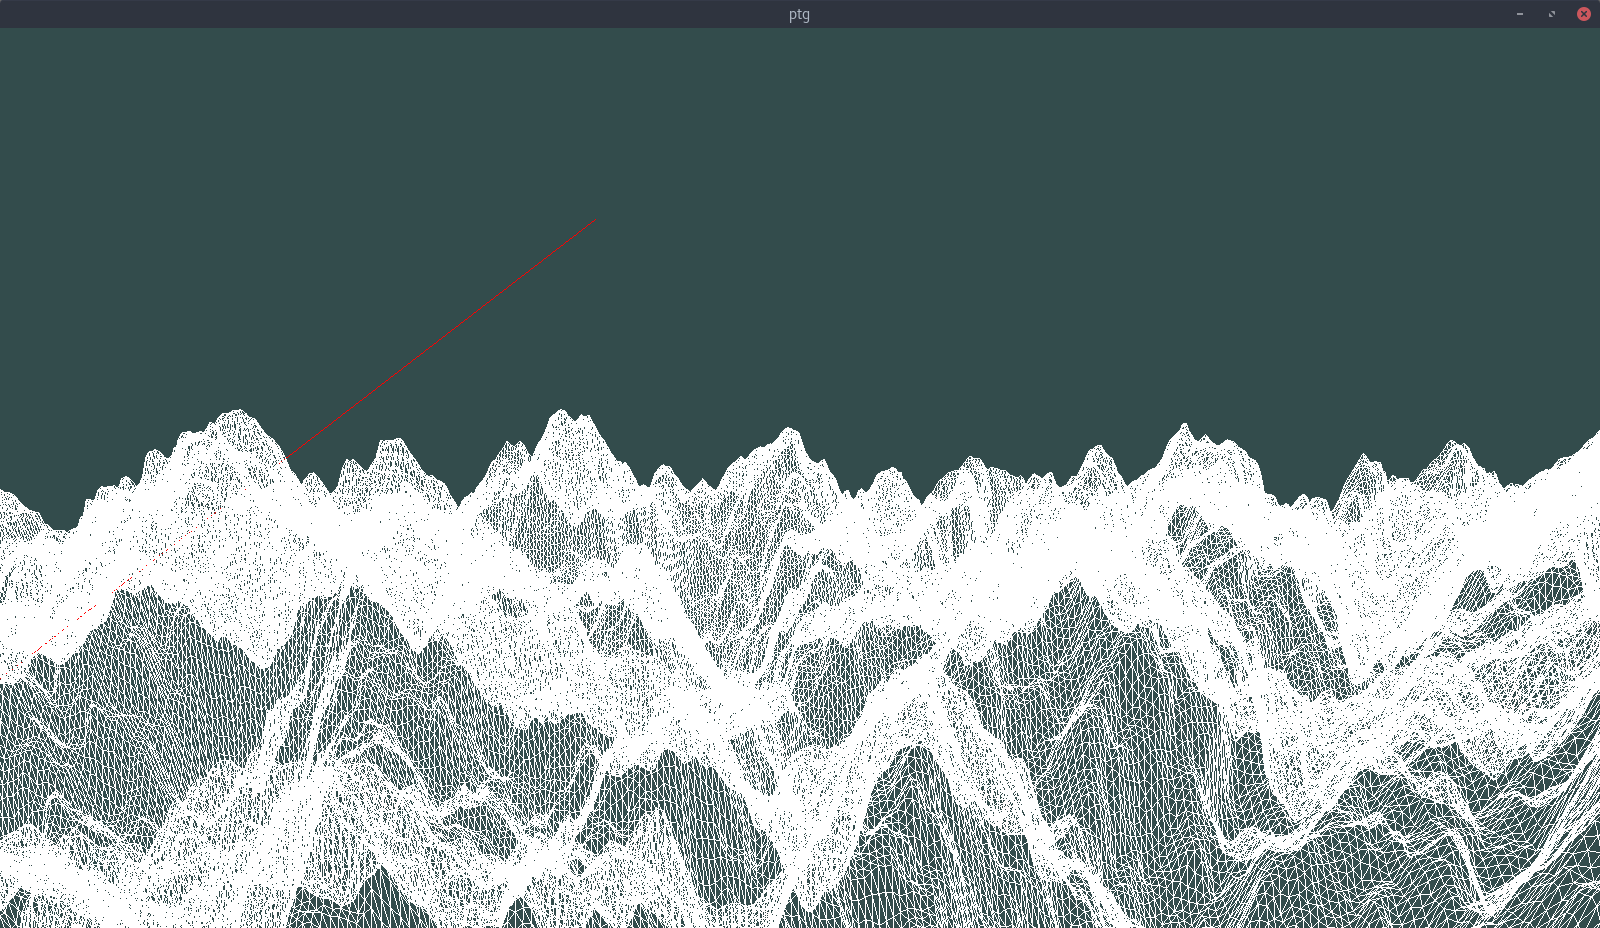
\includegraphics[width=0.3\textwidth]{figuras/freq16.png}\label{fig:freq16}}
     \caption{Comparando influência da frequência.}
     \label{fig:parametrosOctaves}
     % usar \hspace{0.1cm}, é gambiarra mas funciona
\end{figure}

Usando $f = 8, amp = 30$ e $Octaves = 8, seed = 15$ e variando a seed.

\begin{figure}[H]
     \centering
     \subfloat[][$seed = 1$]{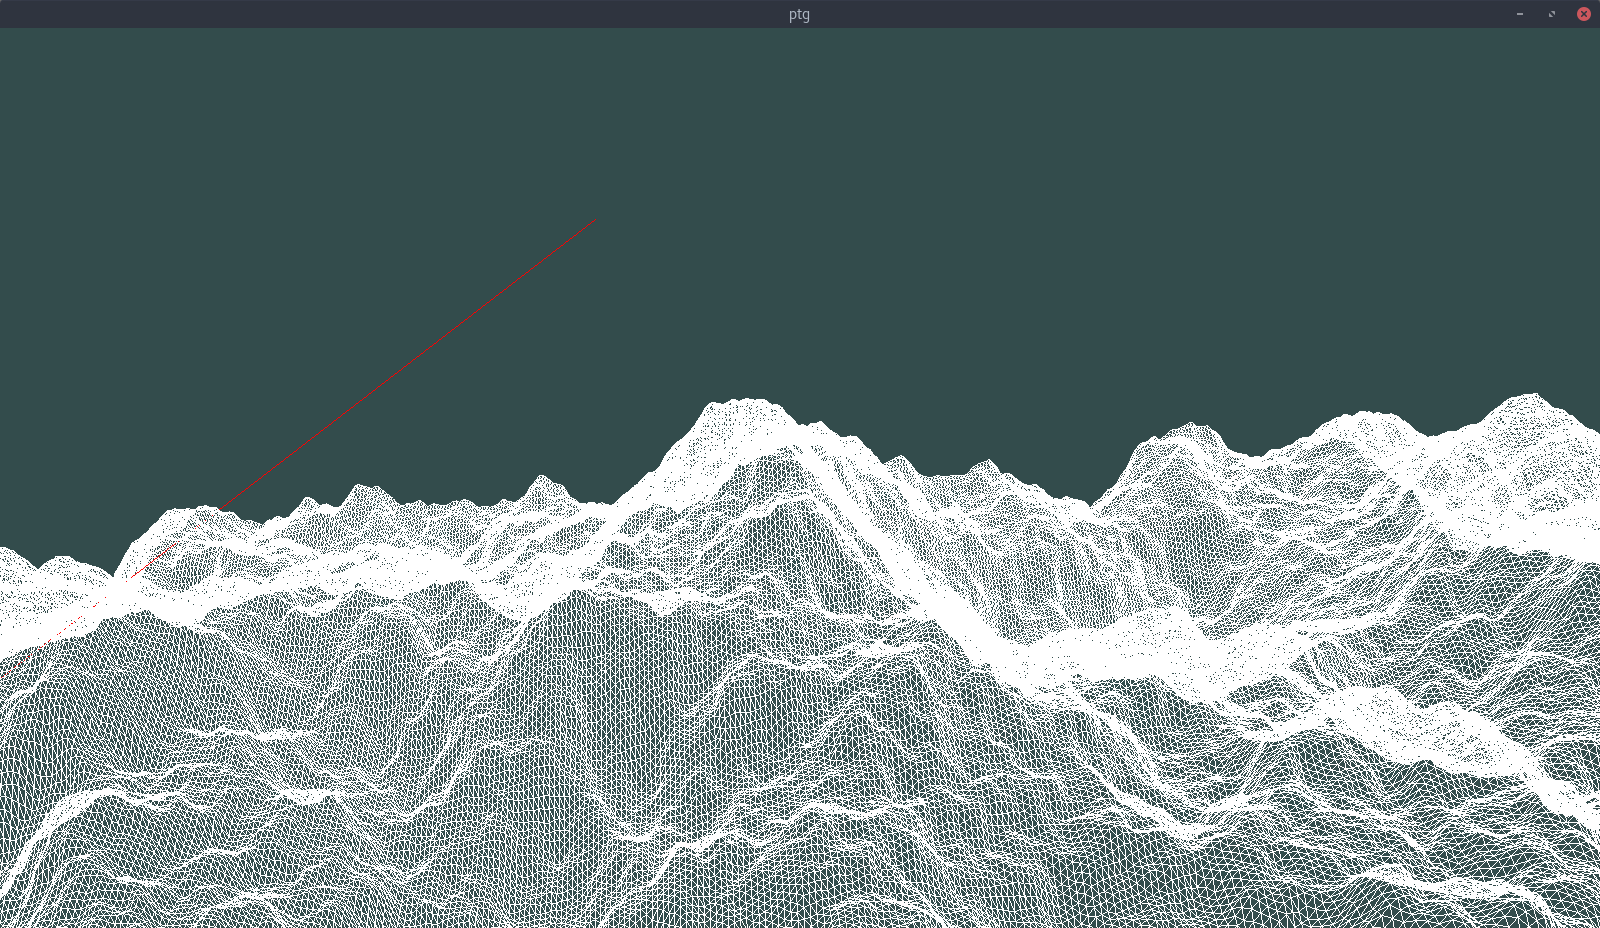
\includegraphics[width=0.3\textwidth]{figuras/seed1.png}\label{fig:seed1}}\hspace{0.1cm}
     \subfloat[][$seed = 2$]{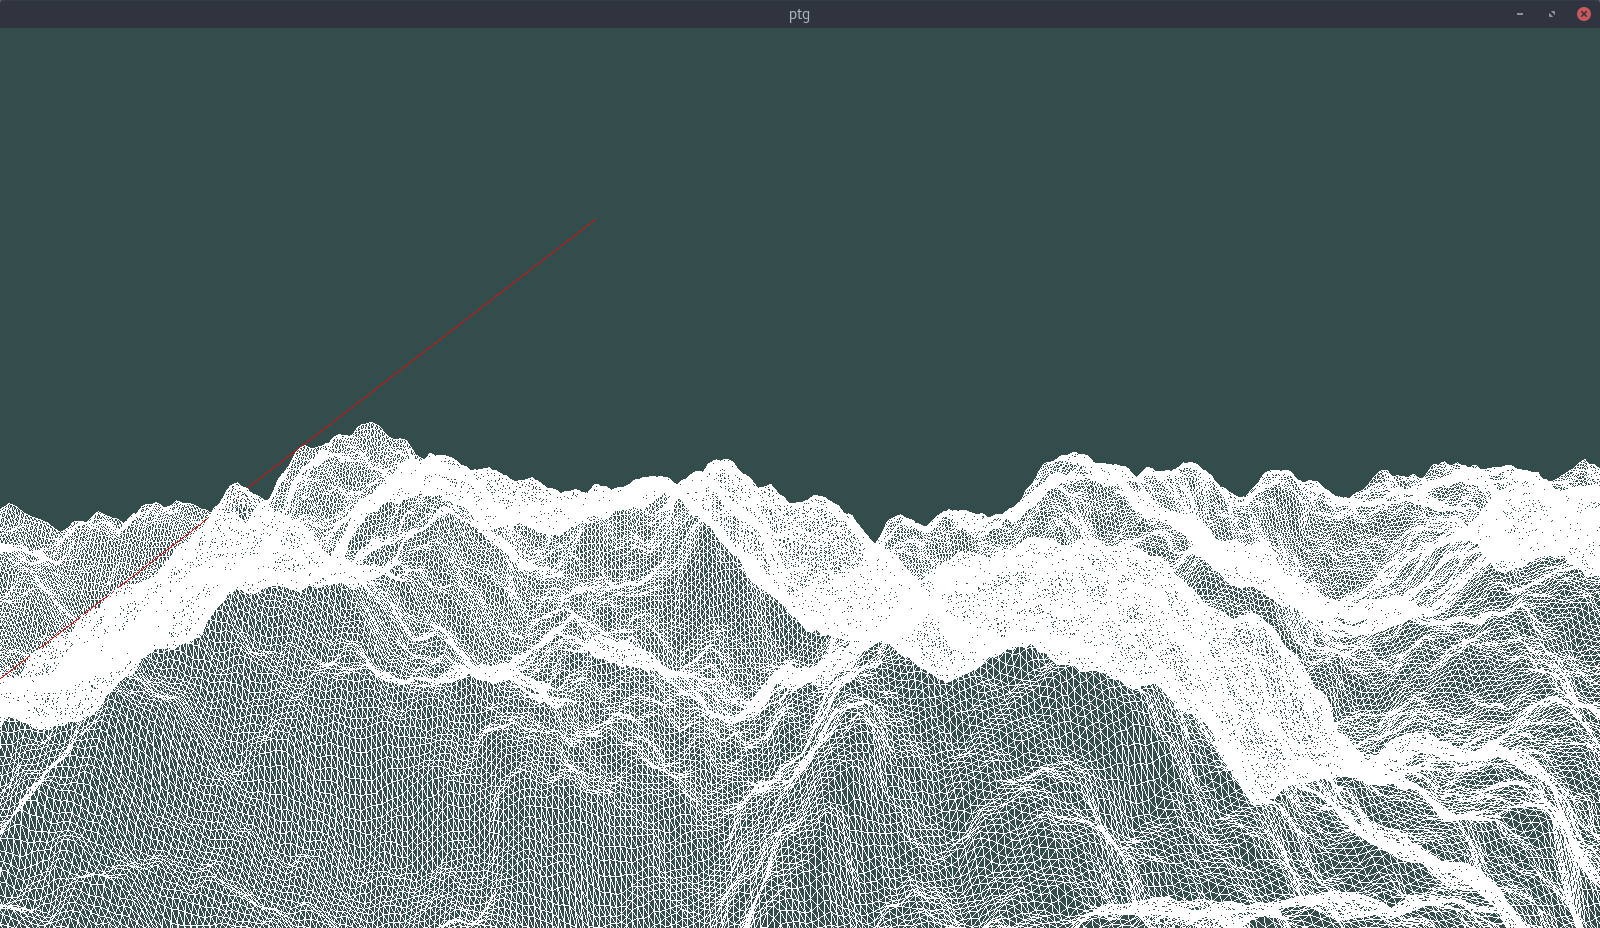
\includegraphics[width=0.3\textwidth]{figuras/seed2.png}\label{fig:seed2}}\hspace{0.1cm}
     \subfloat[][$seed = 3$]{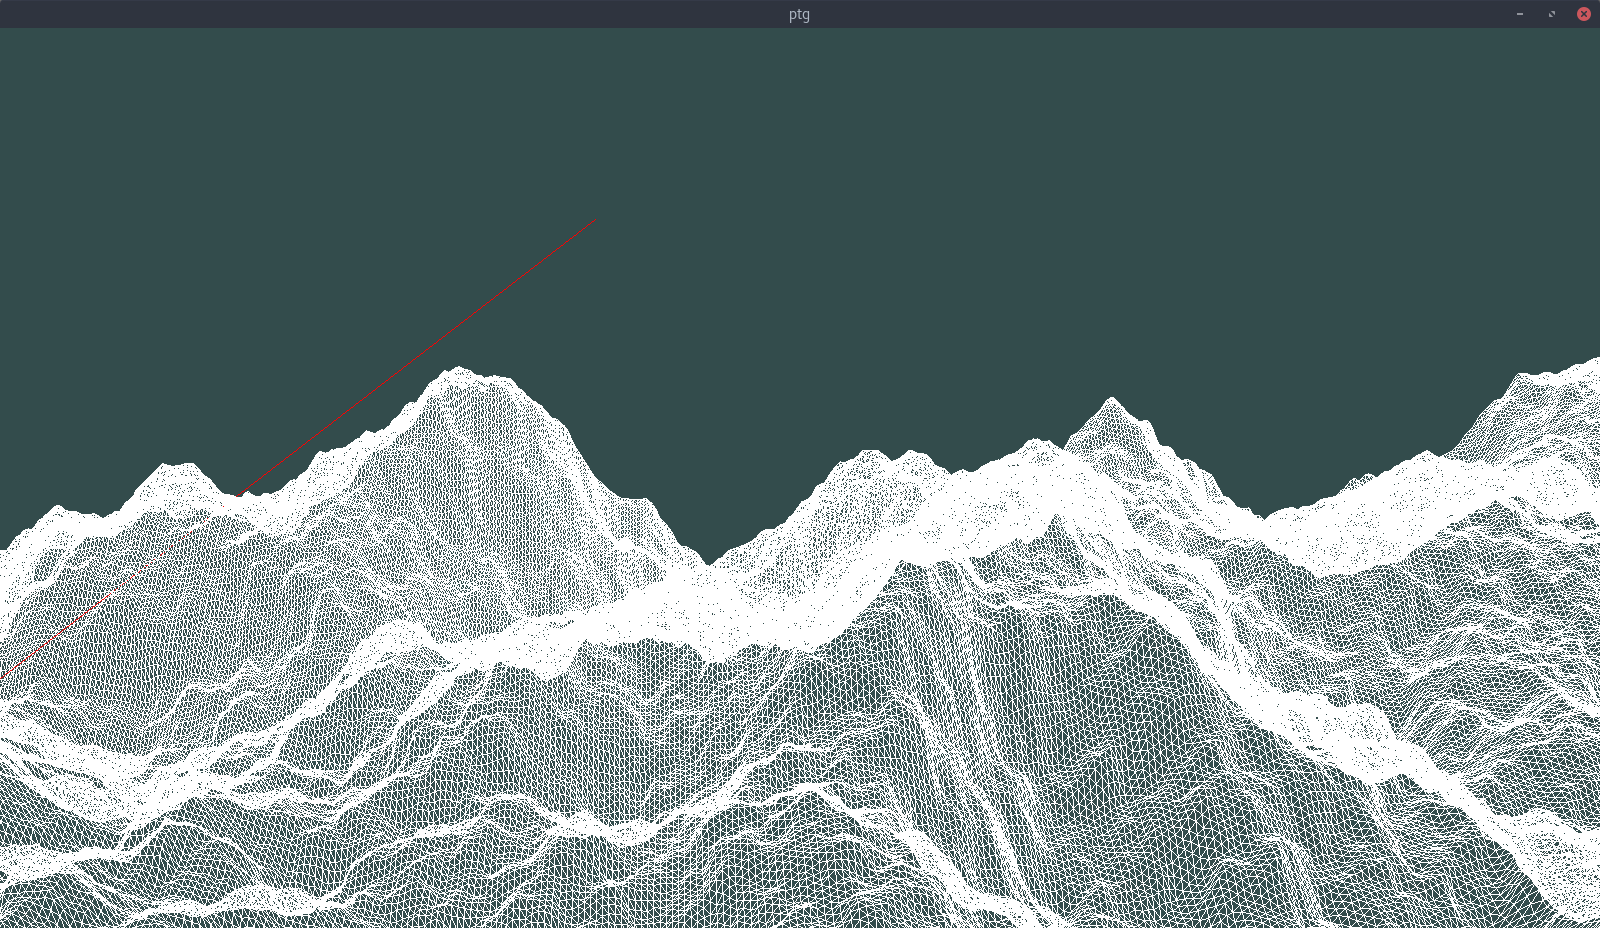
\includegraphics[width=0.3\textwidth]{figuras/seed3.png}\label{fig:seed3}}
     \caption{Comparando influência da seed.}
     \label{fig:parametrosSeed}
     % usar \hspace{0.1cm}, é gambiarra mas funciona
\end{figure}

\subsection{Manipulando ruído para criar Biomas}
\subsubsection{PLAINS}

\begin{figure}[H]
    \centering
    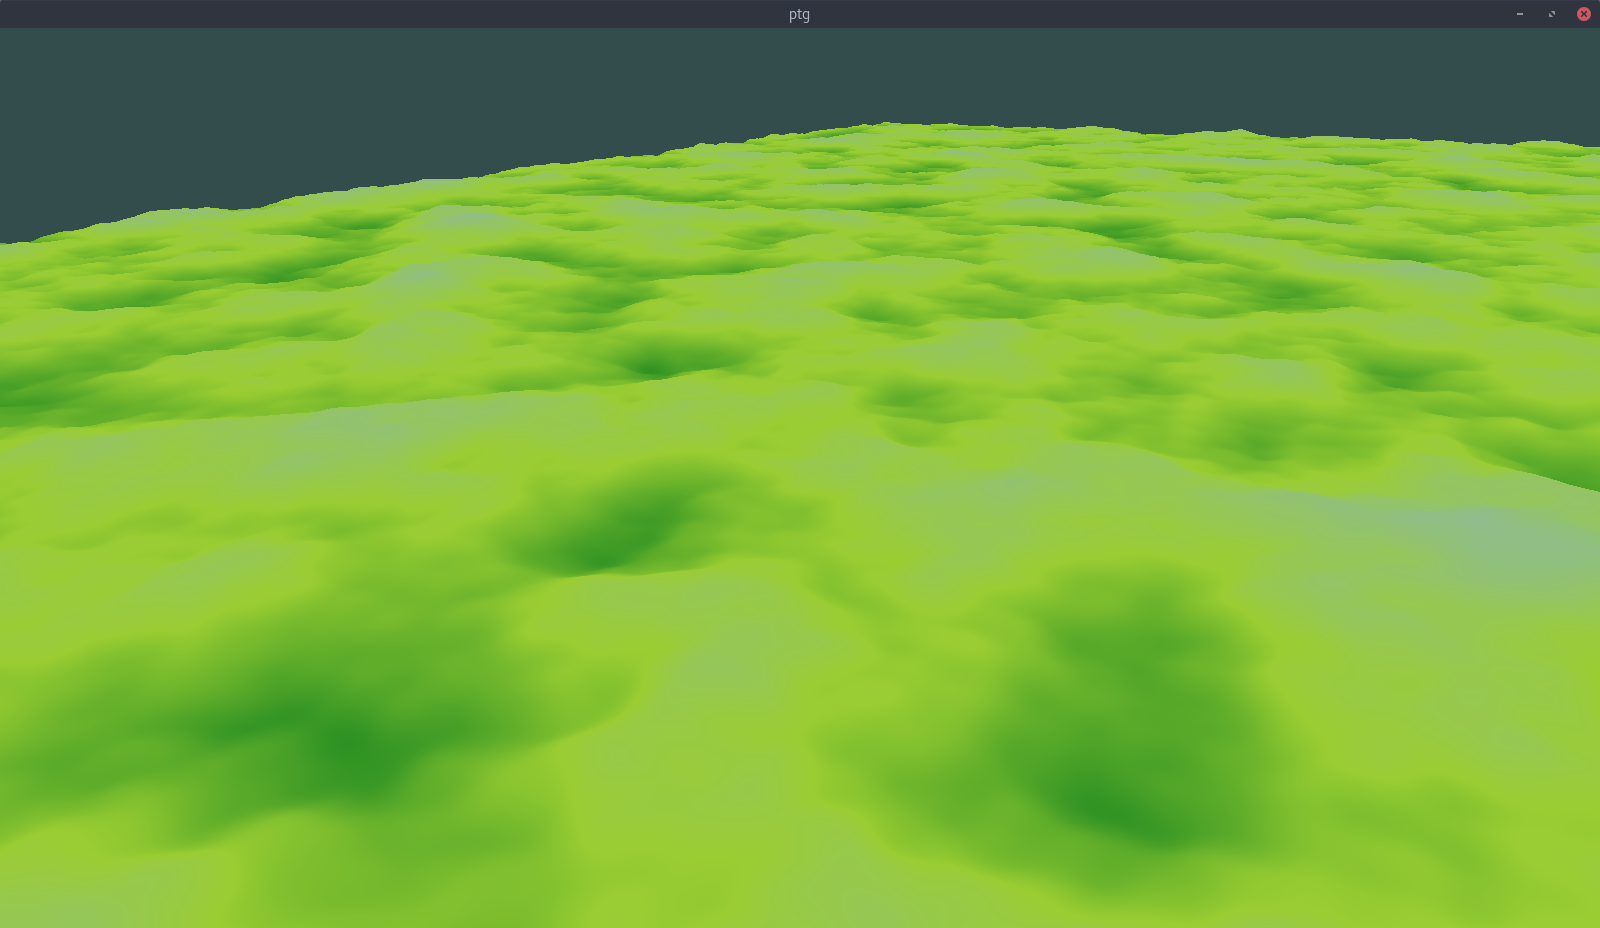
\includegraphics[width=0.5\textwidth]{figuras/bssPlains.png}
    \caption{Consumo}
    \label{fig:bssPlains}
\end{figure}

\subsubsection{MONTAINS}


\begin{figure}[H]
    \centering
    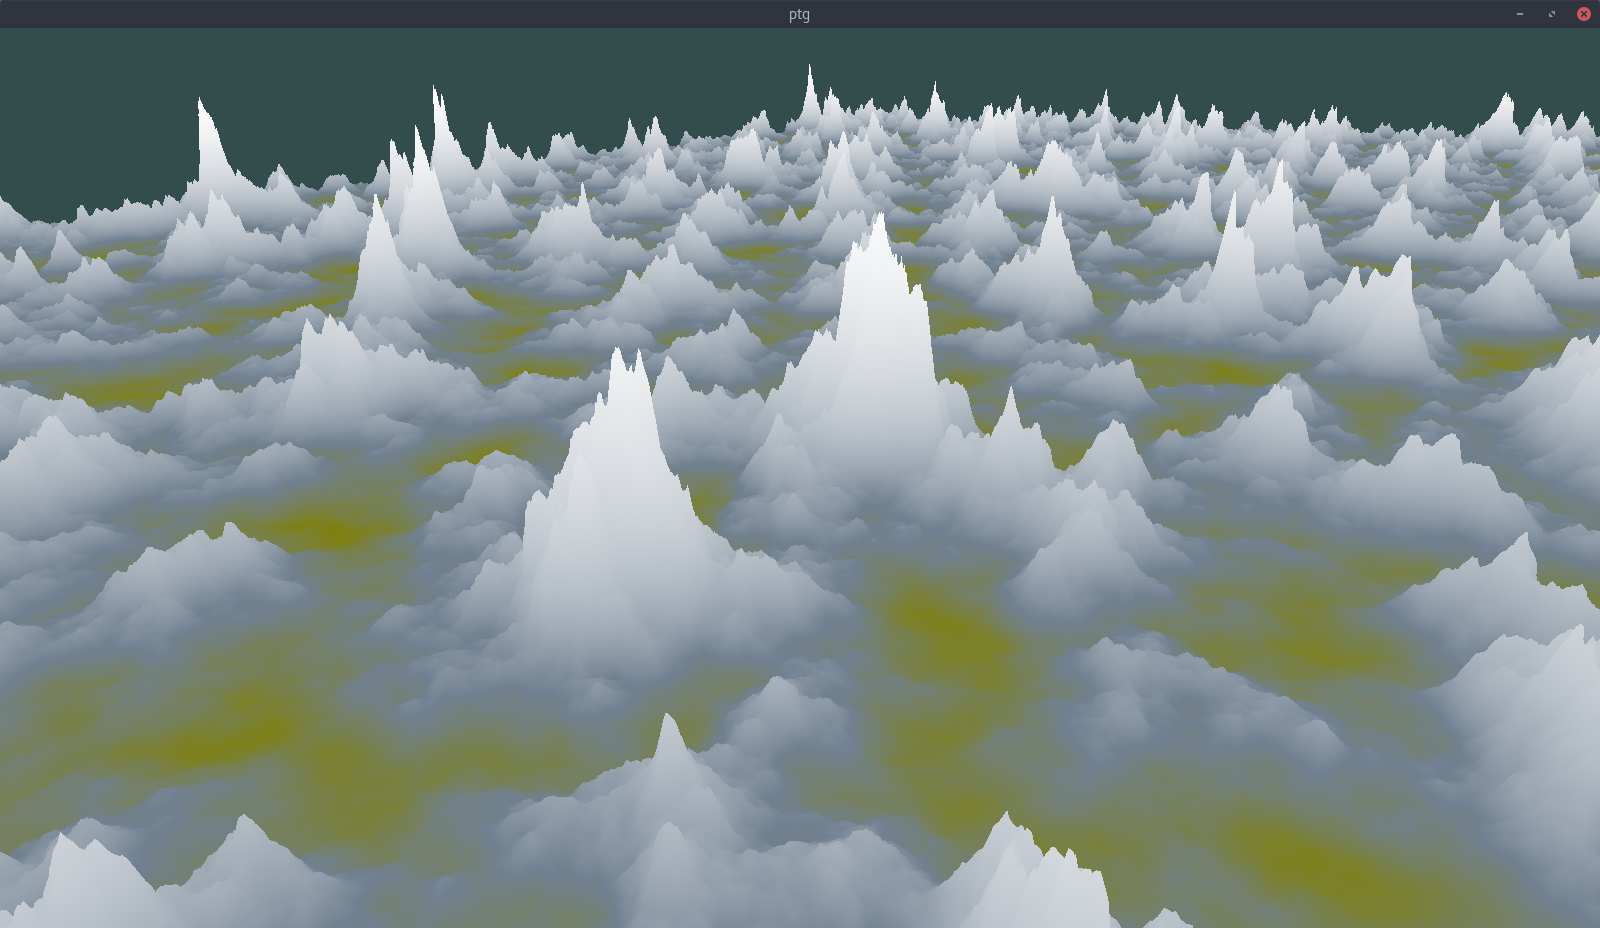
\includegraphics[width=0.5\textwidth]{figuras/bssMontains.png}
    \caption{Consumo}
    \label{fig:bssMontains}
\end{figure}

\subsubsection{VALLEY}


\begin{figure}[H]
    \centering
    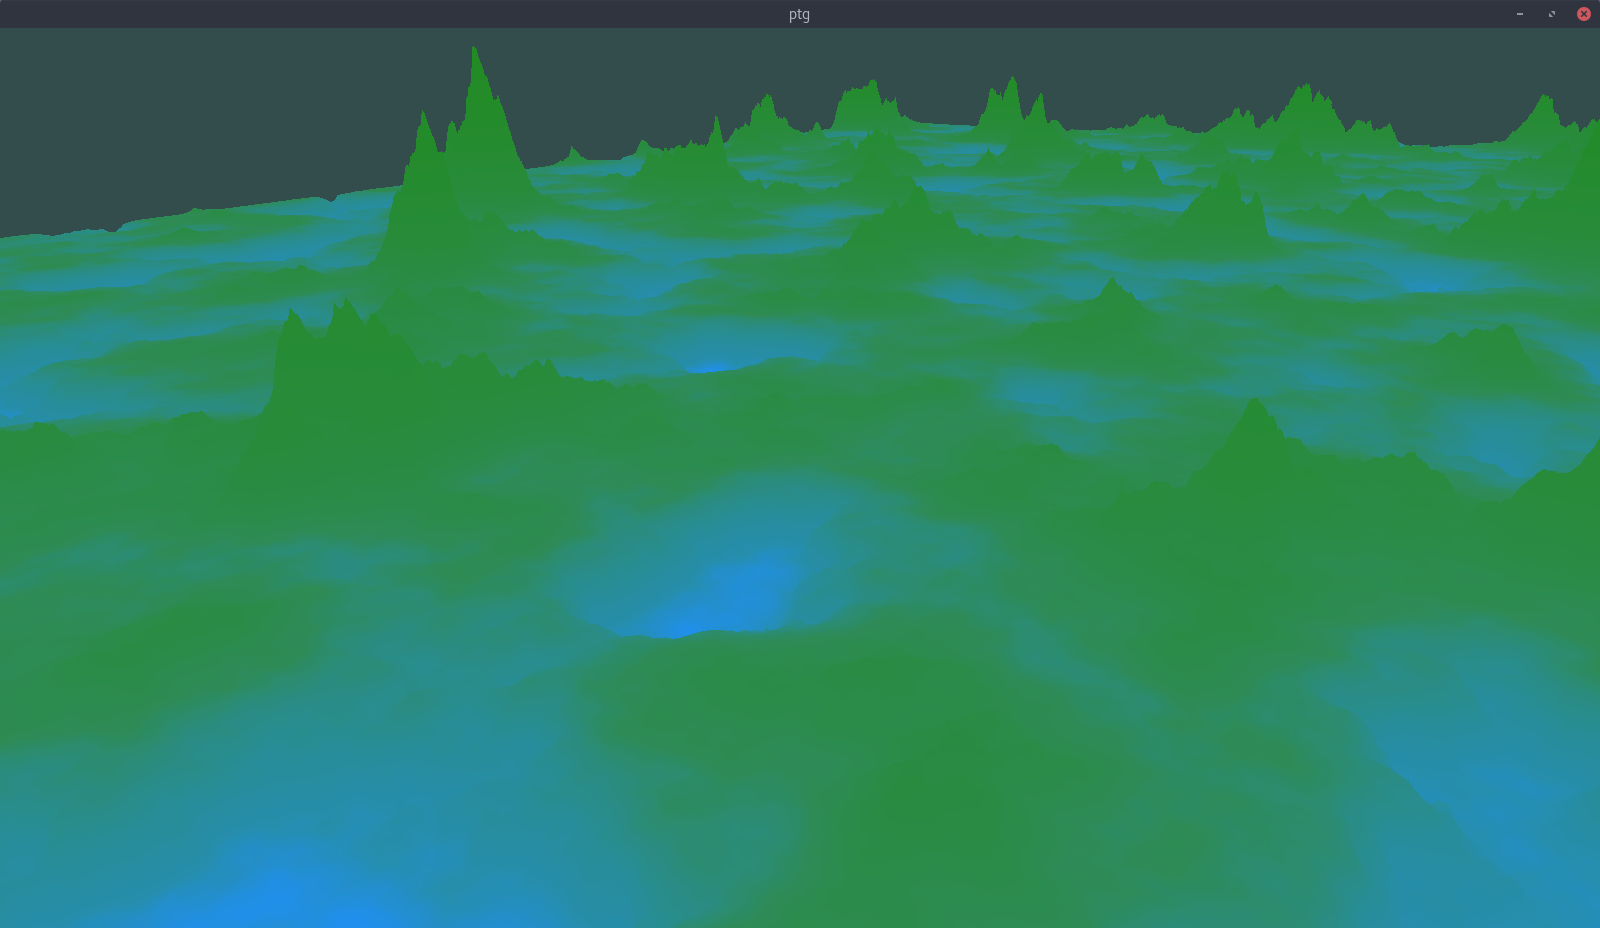
\includegraphics[width=0.5\textwidth]{figuras/bssValley.png}
    \caption{Consumo}
    \label{fig:bssValley}
\end{figure}

\subsubsection{DESERT}


\begin{figure}[H]
    \centering
    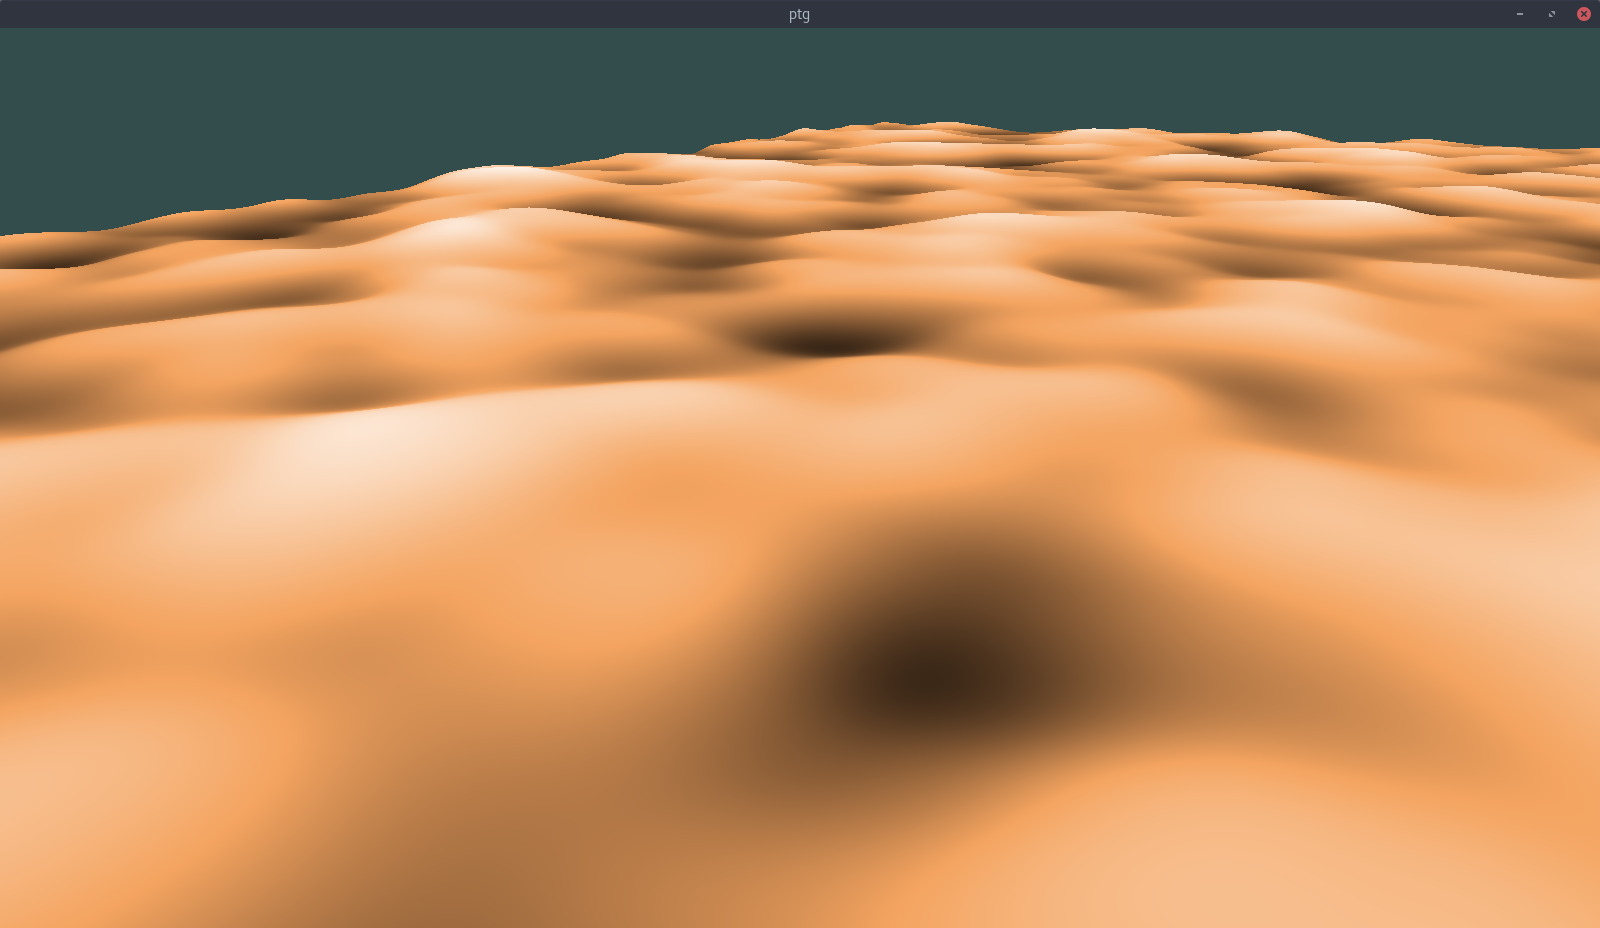
\includegraphics[width=0.5\textwidth]{figuras/bssDesert.png}
    \caption{Consumo}
    \label{fig:bssDesert}
\end{figure}

\subsubsection{CANYONS}


\begin{figure}[H]
    \centering
    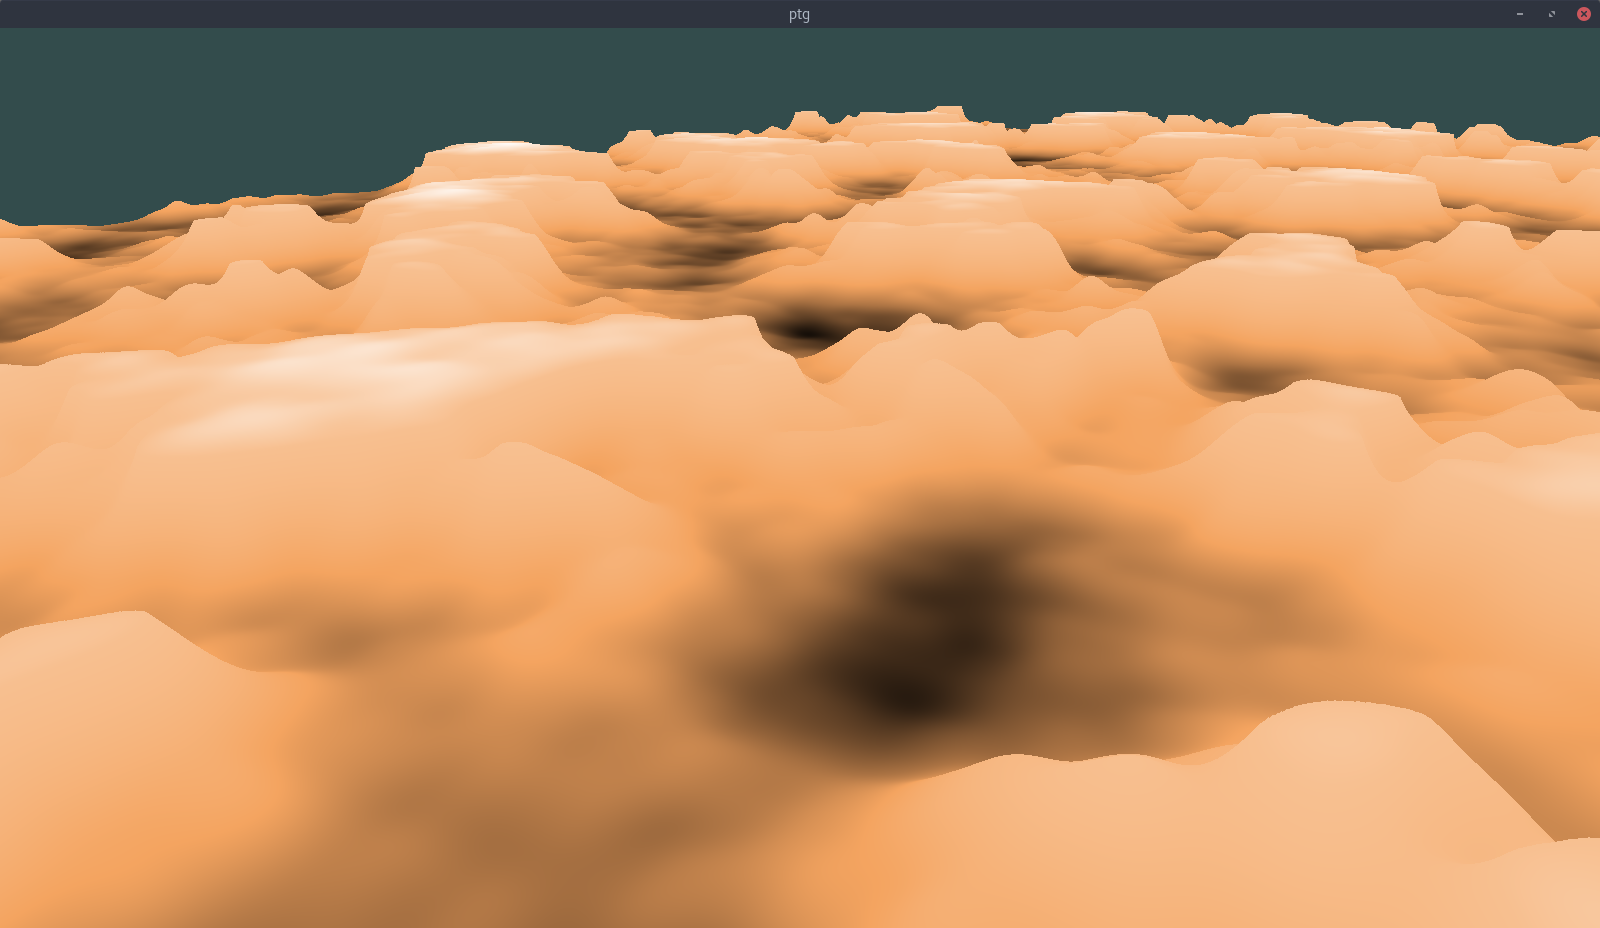
\includegraphics[width=0.5\textwidth]{figuras/bssCanyons.png}
    \caption{Consumo}
    \label{fig:bssCanyons}
\end{figure}

\section{Separando Áreas de Biomas}

\section{Detectando fronteira entre Biomas}